\documentclass[entwurf.tex]{subfiles}

\begin{document}

\chapter{Sequenzdiagramme}
	\section{Terminal connect}
		In dem folgenden Diagramm sieht man den Ablauf vom Verbinden eines Endgeräts mit dem Server bis zur Live-Übertragung der Signale und die Änderung der Anzeigekonfiguration auf dem Endgerät. 
		
		Hierbei handelt es sich beim Terminal um das Endgerät auf dem über einen Browser die Vinjab-Seite aufgerufen wird. Der Befehl openWebpage() vom Terminal zum Webserver nutzt das HTT-Protokoll. 

		Das Hypertext Transfer Protocol (HTTP, englisch für Hypertext-Übertragungsprotokoll) ist ein Protokoll zur Übertragung von Daten auf der Anwendungsschicht über ein Rechnernetz und gehört dementsprechend zur Internetprotokollfamilie. Es wird hauptsächlich eingesetzt, um Webseiten (Hypertext-Dokumente) aus dem World Wide Web (WWW) in einen Webbrowser zu laden. Es ist jedoch nicht prinzipiell darauf beschränkt und auch als allgemeines Dateiübertragungsprotokoll sehr verbreitet. %TODO Referenz, Anhang o.ä.
		
		\begin{figure}[H]
 			\makebox[\textwidth][c]{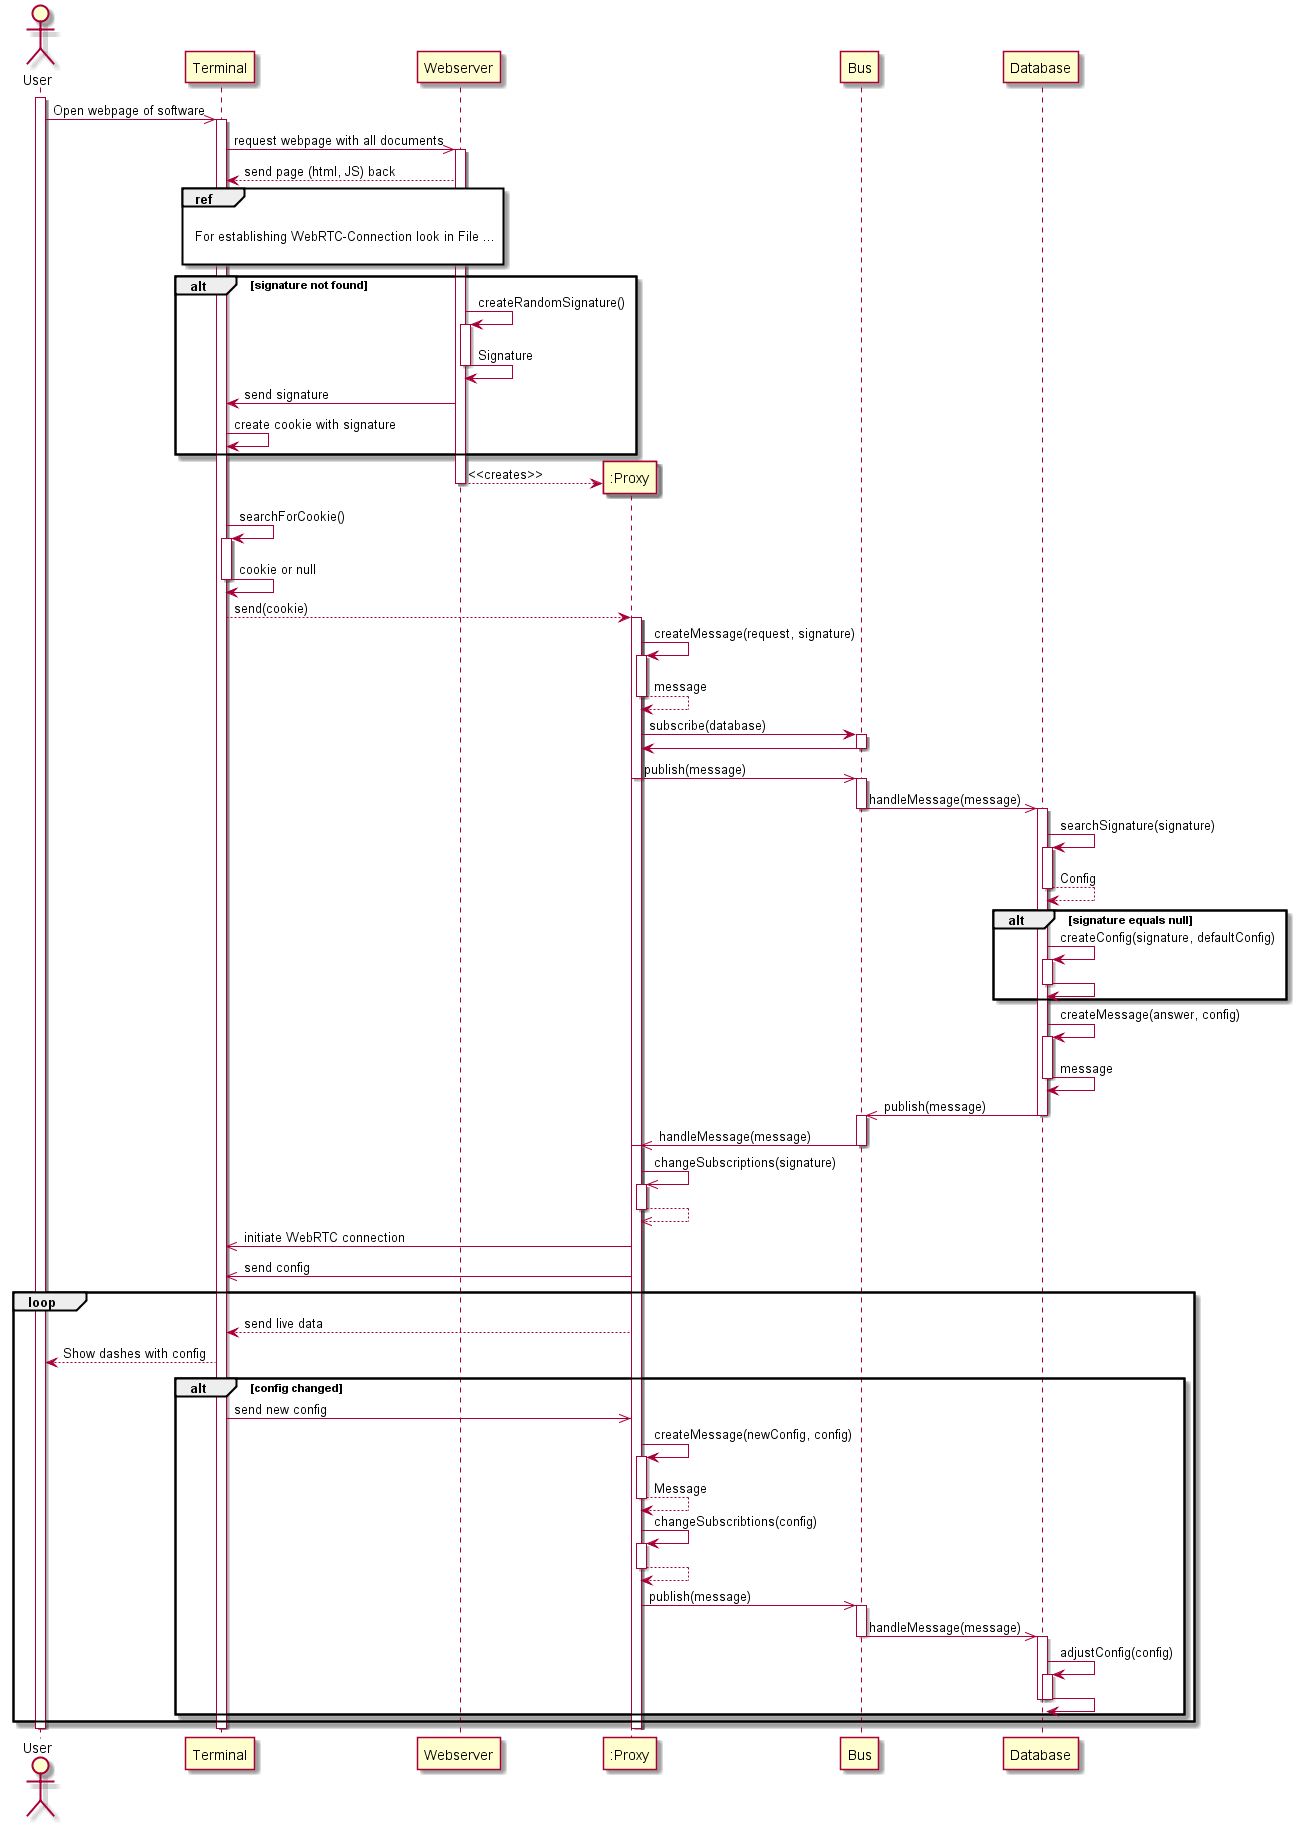
\includegraphics[width=0.9\paperwidth]{diagrams/Connect.png}}
  			\caption{Verschiedene Dash-Anzeigeelemente.}
  		\end{figure}
  		
  	\section{WebRTC connection}
		In dem folgenden Diagramm wird dargestellt wie eine WebRTC-Verbindung zwischen dem Endgerät und dem Webserver hergestellt wird.
		
		WebRTC ist eine Sammlung von Kommunikationsprotokollen und Programmierschnittstellen (API) für die Implementierung in Webbrowsern, die diesen Echtzeitkommunikation über Rechner-Rechner-Verbindungen ermöglichen. Damit können Browser nicht mehr nur Datenressourcen von Backend-Servern abrufen, sondern auch (Echtzeitinformationen) von Browsern anderer Benutzer.
		
		\begin{figure}[H]
			\begin{center}
	 			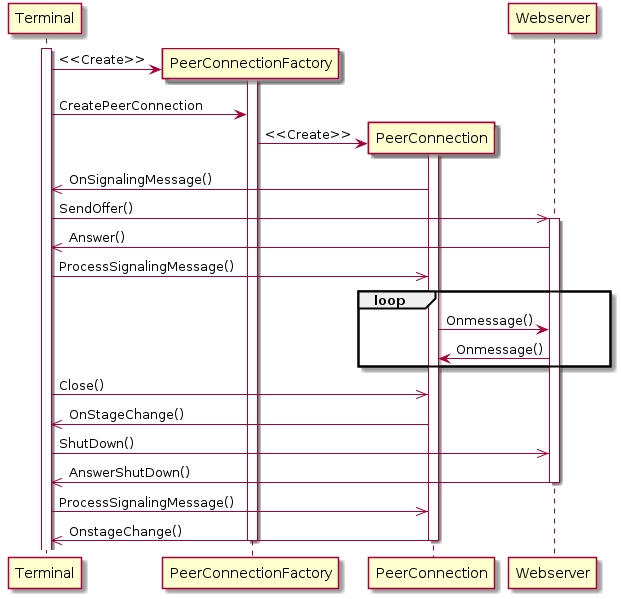
\includegraphics[width=\textwidth]{diagrams/DataTransferSequenz.png}
  				\caption{Verschiedene Dash-Anzeigeelemente.}
  			\end{center}
  		\end{figure}
  		
  	\newpage
  	\section{Changed config}
  		Nach hergestellter Verbindung befindet sich das System in einer Schleife in der eigentlich nur noch Live-Daten vom Server zum Client geschickt wird. Nur wenn die Anzeigeeinstellungen der Dashes geändert wurden 
  		\begin{figure}[H]
  			\begin{center}
 				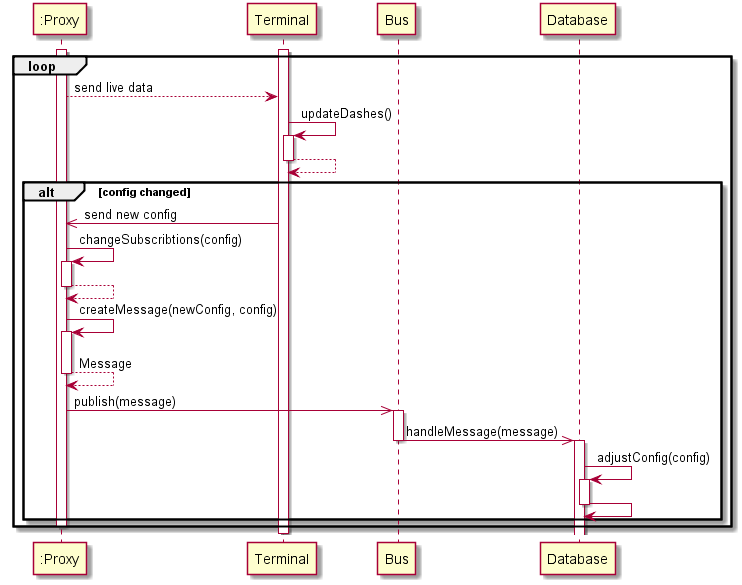
\includegraphics[width=\textwidth]{diagrams/ChangeDashConfig.png}
  				\caption{Verschiedene Dash-Anzeigeelemente.}
  			\end{center}
  		\end{figure}
  		
  	\newpage
	\section{Parkingsensor}
		Der Ablauf beim Start des Parksensors
		\begin{figure}[H]
  			\begin{center}
 				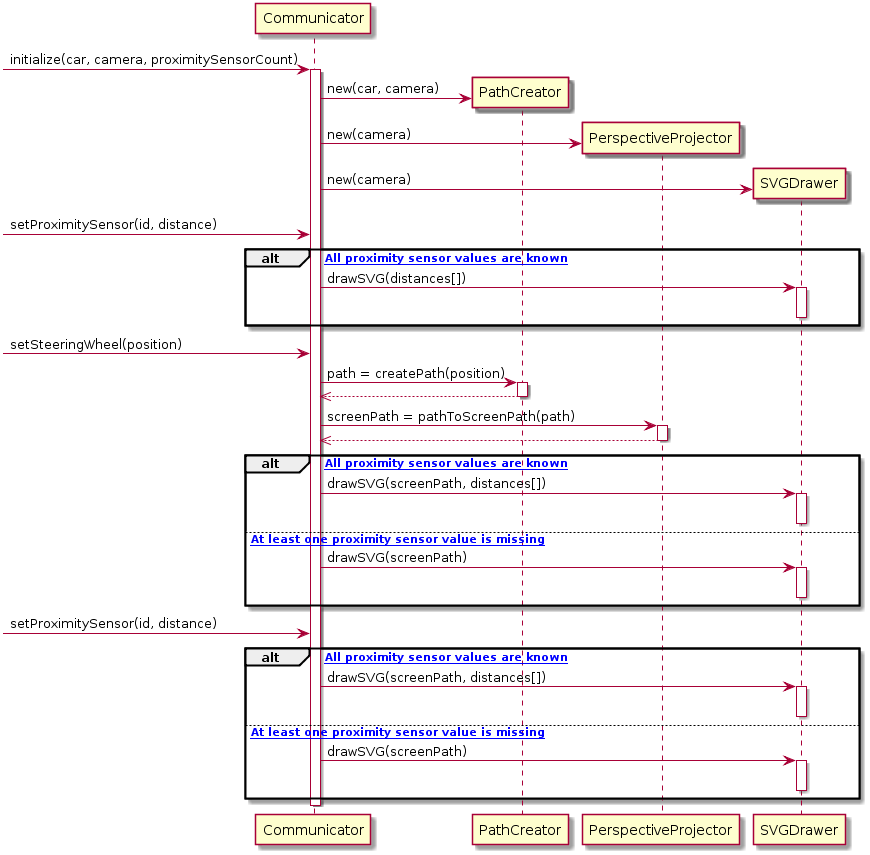
\includegraphics[width=\textwidth]{diagrams/ParkingSensor/sequence_diagram.png}
  				\caption{Verschiedene Dash-Anzeigeelemente.}
  			\end{center}
  		\end{figure}
\end{document}